\documentclass[paper=a4,fontsize=12pt,parskip=half]{scrartcl}

\usepackage{ucs}
\usepackage[utf8x]{inputenc}
\usepackage[T1]{fontenc}
\usepackage{graphicx}
\usepackage{titlesec}
\usepackage{listings}
\usepackage{xcolor}
\usepackage{color}
\usepackage{pgf}
\usepackage{enumitem}
\usepackage[ngerman]{babel}
\usepackage[autostyle=true,german=quotes]{csquotes}
\usepackage[acronym,hyperfirst=false]{glossaries}
\usepackage[colorlinks]{hyperref}
\usepackage{acronym}
\usepackage[colorinlistoftodos,prependcaption]{todonotes}
\usepackage{soul}

% Besseres highlighting von Worten
% https://tex.stackexchange.com/questions/343458/
\makeatletter
\if@todonotes@disabled
\newcommand{\hlnote}[2]{#1}
\else
\newcommand{\hlnote}[2]{\todo{#2}\texthl{#1}}
\fi
\makeatother

\titlespacing*{\section} {0pt}{0ex}{0ex}
\titlespacing*{\subsection} {0pt}{0ex}{0ex}
\titlespacing*{\subsubsection} {0pt}{0ex}{0ex}

\lstdefinestyle{CodeView} {
	columns=flexible,
	numbers=left,
	basicstyle=\scriptsize,
	tabsize=3,
	frame=single,
	backgroundcolor=\color{white},
	keywordstyle=\color{blue},
}

\linespread{1.5}

\title{Abschlussarbeit}
\author{Tom Hilge}

\makeglossaries

\newcommand{\JS}{JavaScript}

\newacronym{JWT}{JWT}{JSON Web Token}
\newacronym{URI}{URI}{Uniform Resource Identifier}
\newacronym{HTTP}{HTTP}{Hypertext Transfer Protocol}
\newacronym{CSS}{CSS}{Cascading Style Sheets}
\newacronym{JSON}{JSON}{JavaScript Object Notation}
\newacronym{MVC}{MVC}{Model View Controller}
\newacronym{HTML}{HTML}{Hypertext Markup Language}
\newacronym{DOM}{DOM}{Document Object Model}
\newacronym{SPA}{SPA}{Single Page Application}
\newacronym{CLI}{CLI}{Command Line Interface}
\newacronym{API}{API}{Application Programming Interface}
\newacronym{RFC}{RFC}{Request for Comments}
\newacronym{MIME}{MIME}{Internet Media Type}
\newacronym{HMAC}{HMAC}{Keyed-Hash Message Authentication Code}
\newacronym{SHA256}{SHA256}{Secure Hash Algorithm 256 Bit}
\newacronym{oAuth2}{oAuth2}{Open Authorization 2.0}
\newacronym{UUID}{UUID}{Universally Unique Identifier}
\newacronym{STI}{STI}{Single Table Inheritance}
\newacronym{XSS}{XSS}{Cross-Site-Scripting}
\newacronym{CSRF}{CSRF}{Cross-Site-Request-Forgery}
\newacronym{HTTPS}{HTTPS}{Hypertext Transfer Protocol Secure}
\newacronym{URL}{URL}{Uniform Resource Locator}


\begin{document}

        \tableofcontents
        \clearpage

	\section{Einführung}
	\label{sec:introduction}
	Aktuell ist in Blattwerkzeug keine Benutzer-Authentisierung, -Authentifizierung und -Autorisierung implementiert. Dies hat zur Folge, dass  zum jetzigen Zeitpunkt jeder Blattwerkzeug-Nutzer dazu autorisiert ist, jegliche, vom Client erlaubten\todo{Der Server erlaubt, der Client bietet an}, Änderungen vorzunehmen. Dies resultiert aus dem bisher einzigen Nutzer in der Datenbank. Das Adminpanel ist beispielsweise für jeden Blattwerkzeug-Nutzer, über die Seiten-Navigation, frei zugänglich. Im Rahmen dieser Thesis soll genau dieses\todo{du löst noch mehr} Problem gelöst werden. Nach Behandlung der Thesis soll es möglich sein, sich mit einer standardisierten Registrierung bei Blattwerkzeug anzumelden. Außerdem soll es ebenfalls möglich sein, sich über externe Anbieter anzumelden. Zusätzlich soll je nach Benutzerrolle und Benutzergruppe des angemeldeten Nutzers unterschiedlicher Inhalt dargestellt werden. Darüber hinaus soll ein angemeldeter Benutzer die Möglichkeit haben sein bereits erstelltes Konto mit weiteren E-Mails oder externen Konten zu verknüpfen. In den Einstellungen soll es dem Nutzer außerdem ermöglicht werden seine verknüpften Konten zu verwalten.

	\section{Technologien}
	\label{sec:technology}
	Im Verlauf dieser Sektion werden die Technologien und deren Verwendungszweck
	kurz erläutert.

	\subsection{Blattwerkzeug}
	\label{sec:blattwerkzeug}

	\begin{figure}
		
\includegraphics[scale=0.4]{images/blattwerkzeug.png}
	\end{figure}


	Blattwerkzeug ist ein quelloffenes Projekt, dass Informatik-Interessierten das Programmieren von \gls{HTML} Grundgerüsten und SQL Statements per \enquote{drag and drop} näher bringen kann. Dabei versteckt Blattwerkzeug die Syntax nicht vor dem Nutzer, sondern gibt ihm die Möglichkeit diesen gleich mit ein zu sehen. Dennoch ist es dem Nutzer einfach gemacht, mit visuellen Elementen teile der Informatik kennen zu lernen.

	Dabei hat es sich Blattwerkzeug vor allem als Aufgabe gemacht an Schulen aufzutreten. Mit Blattwerkzeug wird Lehrern ein Werkzeug in die Hand gelegt, mit dem einfacher und informativer Informatik Unterricht gestaltet werden kann. Somit kann der veraltete und doch sehr Office-lastige Informatik Unterricht komplett erneuert und interessanter gestaltet werden\todo{Zuviel: BlattWerkzeug ist ein Zusatz, keine Ersetzung}.

	\subsection{Passwort Hashing}
	\label{sec:password_hashing}

	Sobald eine Software mit Nutzerdaten geführt wird, ergibt sich das Problem des Speicherns der Passwörter jeweiliger Nutzer.
	Denn sollten die Daten der Nutzer im Klartext in der Datenbank gespeichert werden und ein Angreifer erlangt Zugriff auf die Datenbank, so ist es für ihn ein leichtes weitere Konten der Nutzer zu infiltrieren. Der Grund dafür sind die anwendungsübergreifenden, vom Nutzer größtenteils identischen, Passwörter.

        \todo[inline]{Nicht nur Super-GAU für eigene Seite, sondern auch für Nutzer auf anderen Seiten. Konkretes Beispiel ergänzen (Liesschen Müller ist mit ihrer EMail
          \enquote{lieeschen@müller.de} und dem Passwort \enquote{Milch} bei \enquote{Milchkanne.de} registriert, ...}

	An diesem Punkt kommt das Hashen von Passwörtern zum Einsatz. Passwort Hashing soll dem Nutzer Sicherheit gewährleisten und es einem Angreifer nicht möglich machen mit erlangten Daten weitere Konten der Nutzer zu infiltrieren. Dabei wird aus einem Passwort ein Hash generiert\todo{.}, dieser Hash macht es einem unmöglich, das Passwort wiederherzustellen. Jedoch ergibt sich bei gleicher Eingabe, der gleiche Hash. Um ein gehashtes Passwort zu erhalten, muss ein Hashing Algorithmus auf das jeweilige Klartext Passwort angewendet werden.

	Mittlerweile gibt es verschiedene Hash-Funktionen\todo{Satz führt nirgendwo hin}. Rainbowtables in denen Hashes mit dazugehörigem Klartext Passwort stehen sorgen jedoch dafür, dass manche dieser Hash-Funktionen als nicht mehr riches\todo{?} gelten. Dies hat zur Folge, dass eine Sicherheitslücke ensteht falls ein Angreifer die Nutzerdaten erlangt und die Passwörter mit einer solchen Hash-Funktion gehasht wurden. Die Möglichkeit besteht das gehashte Passwort mit einer Rainbowtable abzugleichen und dabei das jeweilige Klartext Passwort zu erhalten. Weshalb MD5~\ref{fig:md5} und SHA zwei der bekanntesten Hash-Funktionen, seit geraumer Zeit nicht mehr zum Passwort hashen verwendet werden \todo{Stattdessen?}.

	\begin{figure}[h]
		\includegraphics[width=\textwidth]{images/hash-md5.png}
		\caption{Resultat einer MD5 Hashfunktion auf ein Klartext.}
		\label{fig:md5}
	\end{figure}

	\begin{figure}[h]
		\includegraphics[width=\textwidth]{images/rainbowtable.png}
		\caption{Beispiel einer Rainbowtable.}
		\label{fig:rainbowtable}
	\end{figure}

	Aus diesem Grund werden sogenannte Salts~\ref{fig:salted-hash}, zufällig generierte Zeichenketten, an das Passwort angehängt und darauffolgend die Hashfunktion angewandt.

        \todo[inline]{Beispielhafte Datenbanktabelle?}

	\begin{figure}[h]
		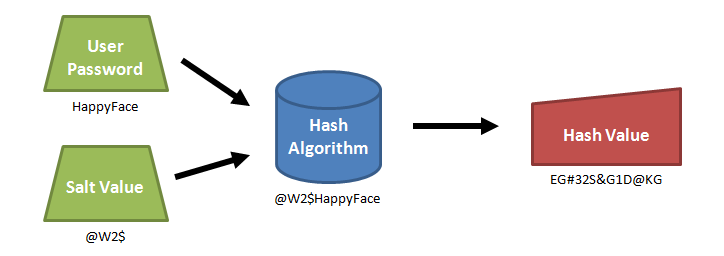
\includegraphics[width=\textwidth]{images/salted_hash.png}
		\caption{Hashfunktion auf Klartext und Salt angewandt.}
		\label{fig:salted-hash}
	\end{figure}

	\subsection{Sessions}
	\label{sec: sessions}

	Das \gls{HTTP} ist ein zustandsloses Protokoll, dass sich keine Informationen der jeweiligen Aufrufe zwischenspeichert. Dies ist unpraktisch\todo{In vielen Fällen ist das auch praktisch}, da so keine Informationen des Nutzers kurzzeitig gespeichert werden können. Ein Verwendungszweck wäre beispielsweise der Warenkorb, da dieser nur temporär vorhanden sein soll. Genau dieses Problem kann mit der Session gelöst werden\todo{Warum lösen Cookies das Problem nicht?}.

	Die Session ist eine serverseitige Daten-Speichermöglichkeit. Dabei wird bei der Anfrage von einem Client an den Server ohne Session-ID eine Session und Session-ID erstellt. Diese Session-ID wird bei der Antwort des Servers mit an den Client ausgeliefert. Ab diesem Punkt wird bei jeder Anfrage vom Client an den Server die Session-ID mit gesendet. Dies kann über einen Cookie oder über die \gls{URI} erfolgen. Aufgrund dessen kann der Server dem Client Daten aus der jeweiligen Session zur Verfügung stellen.

	IMAGE

	\subsection{JSON Web Token}
	\label{sec: jwt}
	\enquote{\gls{JWT} sind auf \gls{JSON} basierende \gls{RFC} 7519 genormte Access-Token.} \gls{RFC} ist eine Sammlung aus Dokumenten in denen das Verhalten der Technologien des Internets beschrieben ist. Einige davon gehören zum Standard und werden somit in den meisten Fällen vorausgesetzt. In speziellen Fällen möchte beispielsweise ein Unternehmen eigene Protokolle verwenden die nicht zum Standard gehören.

	Diese Tokens werden zur eindeutigen Identifizierung von Nutzern verwendet und können die Session ersetzen. Dabei ist es bei einem \gls{JWT} nicht vonnöten die Daten auf dem Server zu speichern. Dies hat zur Folge, dass die Pflege des Speichers an diesem Punkt entfällt. Jedoch haben \gls{JWT} einen großen Nachteil, sobald der Server einen \gls{JWT} ausgestellt hat, ist dieser bis zum Ablauf des Tokens gültig. Das heißt, sollte ein Server die Berechtigung eines Nutzers nach Ausstellung eines \gls{JWT} ändern, ist diese Änderung erst bei erneutem Erstellen eines \gls{JWT} gültig.

	Ein \gls{JWT} besteht aus Header, Payload und Signatur. Dabei ist der Header und die Payload jeweils ein \gls{JSON} Objekt.

	\subsubsection{Header}
	\label{sec: jwt_header}

	\begin{description}
		\leftskip=1em
		\item[typ] Der typ Claim beschreibt den \gls{MIME} des \gls{JWT}, dieser wiederum teilt dem Client oder Server mit um welche Art von Medium an Daten es sich handelt. Der Standardwert dieses Claims beläuft sich auf \enquote{JWT}, übersetzt \enquote{application/jwt}.
		\item[alg] Der alg Claim beschreibt die Verschlüsselungsmethode. Ein Beispiel ist \gls{HMAC} mit \gls{SHA256}, HS256 abgekürzt.
	\end{description}

	\begin{figure}[h]
		\includegraphics[width=\textwidth]{images/jwt-header.png}
		\caption{Beispiel eines \gls{JWT} Headers }
		\label{fig:jwt-header}
	\end{figure}

	\subsubsection{Payload}
	\label{sec: jwt-payload}

	Die Payload beinhalteten Schlüssel-Wert Paare werden Claims genannt. Dabei handelt es sich um ein JSON Objekt, bei dem bestimmte Schlüssel des Objektes bereits reserviert sind. Diese nennen sich registrierte Claims. Außerdem gibt es öffentliche und private Claims. Hierbei wird zwischen öffentlichen und privaten differenziert.

	\noindent
	\textbf{Beispiel registrierter Claims}

	\begin{description}
		\leftskip=1em
		\item[iss]
		Der iss Claim steht für den Austeller des Tokens, beispielsweise eine Domain.
		\item[exp] Der exp Claim kennzeichnet den \gls{JWT} mit einem Ablaufdatum.
	\end{description}

	\todo[inline]{Mehr konkrete Beispiele, weniger Breite}

	\noindent
	\textbf{Öffentliche Claims}

	Öffentliche Claims sind zusätzlich zum Standard nutzbar und ihre Namen sollten Semantisch dem dazugehörigen Wert entsprechen. Außerdem sollten die Namen der Claims Netzwerkübergreifend verständlich sein.~\ref{fig:public-claim}

	\noindent
	\textbf{Private Claims}

	Private Claims werden nur innerhalb eines Netzwerkes verwendet. Aus diesem Grund gibt es keine implizite Beschränkung in der Namensgebung.~\ref{fig:private-claim}

	\begin{figure}[h]
		\centering
		\includegraphics[width=\textwidth]{images/public-claim.png}
		\caption{Öffentlicher Claim eines \gls{JWT} }
		\label{fig:public-claim}
	\end{figure}

	\begin{figure}[h]
		\centering
		\includegraphics[width=\textwidth]{images/private-claim.png}
		\caption{Privater Claim eines \gls{JWT} }
		\label{fig:private-claim}
	\end{figure}

	\subsubsection{Signatur}
	\label{sec: jwt_signature}

	Um die Signatur zu erhalten muss die Payload und der Header Base64 kodiert werden. Außerdem müssen diese beiden kodierten Zeichenfolgen mit einem Punkt als Trennzeichen verknüpft werden. Darauffolgend wird eine Hashfunktion auf das jeweilige Ergebnis mit zusätzlich sicherer Zeichenfolge als Parameter angewandt. Da diese sichere Zeichenfolge, auch Private Key genannt, nur auf dem Server hinterlegt ist, ist es dem Client zwar möglich den \gls{JWT} zu verändern, ihn jedoch mit korrekter Signatur zu versehen nicht.

	\subsubsection{Zusammengesetzes Token}
	\label{sec: jwt_result}
	Schlussendlich ergibt sich der \gls{JWT} aus kodiertem Header, kodierten Payload und der Signatur. Dabei steht der Header am Anfang Abbildung \ref{fig:jwt-encoded} Rot gekennzeichnet. Darauffolgend mit einem Punkt getrennt die Payload und zum Schluss die Signatur, ebenfalls mit einem Punkt getrennt.

	\begin{figure}[h]
		\centering
		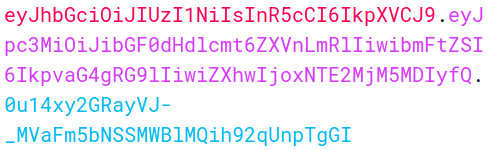
\includegraphics[scale=0.9]{images/jwt-encoded.png}
		\caption{Beispiel eines kodierten \gls{JWT} }
		\label{fig:jwt-encoded}
	\end{figure}

	\subsection{Ruby on Rails}
	\label{sec: rails}
	Ruby on Rails ein quelloffenes Webframework für die Programmiersprache Ruby. Das Webframework nutzt das \gls{MVC} Muster und stellt bereits ein sehr umfangreiches \gls{CLI} zur Verfügung. Mittels des generate Werkzeugs kann beispielsweise Model, View und Controller erstellt werden. Jeder dieser Komponenten wird automatisch in die erstellte Rails Anwendung eingebunden. Außerdem stellt Rails eine umfangreiche Test-Architektur und einen Service zum Versenden von Mails. Dabei kann der Inhalt der E-Mail im Textformat oder als \gls{HTML} versendet werden. Einer der wesentlichen Vorteile von Ruby on Rails ist jedoch die Datenbankanbindung. Hierbei bietet Rails einen Nachhaltigen und Rücksichtsvollen Umgang mit der Datenbank, beispielsweise Migrationen. Migrationen erlauben die Datenbank, ohne explizite SQL-Statements, zu verändern. Außerdem erleichtern Migrationen die Implementierung einer Datenbankstruktur auf einem anderen System.

	\todo[inline]{Nochmal in den eigenen Quelltext schauen: Welche Aspekte sind wirklich relevant?}

	\subsubsection{Routen}
	\label{sec: routen}
	Die Routen in Rails verweisen auf einen Controller und auf eine Funktion innerhalb des Controllers. Dabei wird die Route meistens mit der Anfragemethode eingeleitet, beispielsweise \enquote{get}. Routen können in sogenannte \enquote{scopes}~\ref{fig:routes-scope} unterteilt werden. Somit ist es nicht vonnöten bei einer Verschachtelten \gls{URI} redundant zu werden.~\ref{fig:routes-redundant}

	\begin{figure}
		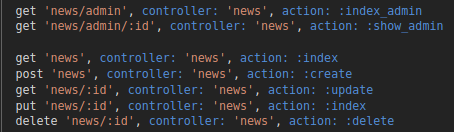
\includegraphics[width=\textwidth]{images/routes-redundant.png}
		\caption{Beispiel einiger redundanter Routen }
		\label{fig:routes-redundant}
	\end{figure}

	\begin{figure}
		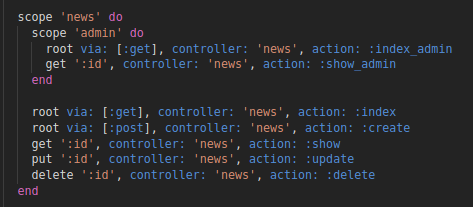
\includegraphics[width=\textwidth]{images/routes-news.png}
		\caption{Beispiel einiger Routen mit scope }
		\label{fig:routes-scope}
	\end{figure}

	\subsubsection{Controller}
	\label{sec: rails_controller}
	Der Controller dient hierbei zur Kapselung von bestimmten Prozessen. Jede Route verweist in irgendeiner Weise auf eine Controller Funktion. In der der jeweiligen Controller Funktion wird dann meistens mit einem Model interagiert. Es wird beispielsweise eine Benutzerberechtigung abgefragt und individuell auf die Berechtigung reagiert. Um auf die jeweilige Berechtigung zu reagieren gibt es mehrere Möglichkeiten. Eine der Möglichkeiten wäre, direkt ein View Template auf dem Server zu rendern und an den Client auszuliefern. Eine andere Möglichkeit wäre ein \gls{JSON} Objekt zurück zu geben und darauf mit dem Client zu agieren.

	\subsubsection{Model}
	\label{sec: rails_model}
	Das Model in Rails stellt jeweils eine Datenbanktabelle dar. Die Attribute des Models sind jeweilige Spalten der Datenbanktabelle. Jeweilige Datenbankeinträge die über das Model erstellt werden, können mittels Validatoren auf ihre Gültigkeit geprüft werden. Diese Validatoren werden innerhalb des Models festgelegt und auf ein Attribut des Models zugewiesen. Rails bietet dabei bereits verfügbare Validatoren, beispielsweise \enquote{presence: true} \hlnote{IMAGE-REF}{Bild Referenz}. Dieser Validator sorgt für das Vorhandensein eines Wertes ungleich \textit{nil}. Jedes Model kann zusätzliche Funktionen beinhalten, die direkt auf den jeweiligen Datenbankeintrag angewandt werden kann. Außerdem bietet Rails die Möglichkeit die Beziehungen zwischen Datenbanktabellen direkt in den Modellen festzulegen.

	\subsubsection{View}
	\label{sec: rails_view}
	Die View stellt in Rails die Möglichkeit \gls{HTML} Template auf dem Server zu rendern. Dabei kann beim rendern das \gls{HTML} Template dynamisch verändert werden. Da diese Komponente während dieser Thesis keine Rolle gespielt hat, wird diese nicht weiter erläutert.

	\subsection{Zusammenfassung}
	\label{sec: rails_resuemee}
	Schlussendlich wird über die Route auf den jeweiligen Controller zugegriffen. Dieser fragt in den meisten Fällen nach einem bestimmten Eintrag eines Models. Darauffolgend wird mit dem Ergebnis der Anfrage interagiert. Es werden Veränderungen oder abfragen bestimmter Daten getätigt. Danach wird ein Ergebnis dem Client ausgeliefert.

        \todo[inline]{Grafik mit Routen, Controllern, Models}



	\subsection{Angular}
	\label{sec: angular}
	Angular ist ein TypeScript basiertes Front-End Webframework, dass in vielen Fällen für \gls{SPA} verwendet wird. \gls{SPA}s laden ihren Inhalt lediglich in ein einziges \gls{HTML} Dokument. Der Inhalt dieses \gls{HTML} Dokumentes wird dynamisch, von beispielsweise einem Framework wie Angular, verändert. Der wesentliche Vorteil von Angular sind die klaren Entwurfsmuster. Jede Komponente in Angular hat im wesentlichen die gleiche Struktur. Dies hat zur Folge, dass Angular eine sehr gute Codekonsistenz bietet.


	\subsubsection{Component}
	\label{sec: ang-component}
	Komponenten in Angular bieten die Möglichkeit \gls{HTML}, \gls{CSS} und TypeScript zu kapseln. Das bedeutet, dass jede Komponente unabhängig von einer anderen Komponente arbeiten kann.

	\subsubsection{Services}
	\label{sec: ang-service}
	Zur Kommunikation mit einem Server und/oder zum Datenaustausch zwischen unterschiedlichen Komponenten wird meistens ein Service verwendet. Jedoch bei einem Datenaustausch zwischen Eltern- und Kind-Komponente ist es einfacher dies mittels der Kind-Komponente durchzuführen. Services werden beim laden der Module instanziiert und dem Konstruktor der Komponente als instanziiertes Objekt übergeben.

	\subsubsection{Module}
	\label{sec: ang-modul}
	Zusätzlich bietet Angular außerdem die Möglichkeit eigene Module zu erstellen in denen dann beispielsweise Services und Komponenten zusätzlich abgekapselt werden können. Ein Vorteil von Angular gegenüber anderen JavaScript Frameworks, sind die bereits von Angular mitgelieferten Module, beispielsweise das Routing- oder das HTTP-Modul. Das Routing-Modul wird für jegliche Navigation auf der Anwendung genutzt. Das \gls{HTTP}-Modul hingegen bietet die Möglichkeit mittels jeglicher Anfragemethoden, mit dem Server zu kommunizieren.

	\subsection{oAuth2}
	\label{sec: oauth2}
	\gls{oAuth2} ist ein offenes \gls{RFC} 6749 Protokoll welches verwendet wird um eine Authentifizierung einer Anwendung mittels Drittanbieter zu ermöglichen. Hierbei wird der Nutzer zuerst auf die jeweilige Seite des Drittanbieters weitergeleitet. Dort muss der Nutzer sich authentifizieren und den Zugriff auf die Daten seines Kontos bestätigen. Nachdem der Zugriff auf die Daten bestätigt wurde, erhält die jeweilige Anwendung von dem Drittanbieter einen Autorisierungs-Token. Dieser Autorisierungs-Token wird darauffolgend von der Anwendung genutzt um einen Zugriffs-Token von dem Drittanbieter zu erhalten. Dieser ermöglicht schlussendlich den Zugriff auf die spezifischen Nutzerdaten des Drittanbieters.~\ref{fig:oauth2}

	In Blattwerkzeug wird genau dieser umfangreiche Vorgang von Omniauth übernommen. Aus diesem Grund wird oAuth2 in dieser Thesis nicht weiter erläutert.

	\begin{figure}[h]
		\includegraphics[width=\textwidth]{images/oauth2.png}
		\caption{oAuth2 verfahren}
		\label{fig:oauth2}
	\end{figure}

	\subsection{Omniauth\todo{Später}}
	\label{sec:omniauth}
	Omniauth ist eine quelloffene Library für Ruby on Rails und ermöglicht einem, eine Anmeldung mittels unterschiedlicher Anbieter über \gls{oAuth2}. Bei der Anmeldung mittels oAuth2 werden bereits viele Funktionen von Omniauth selber übernommen. Sobald der Nutzer sich bei dem jeweiligen Anbieter angemeldet hat, wird die Antwort des jeweiligen Anbieters automatisch über die von Omniauth festgelegte Route verarbeitet. Jedoch muss vorher das spezifische Gem des Anbieters für Omniauth installiert werden. Hierbei stellt jedes Gem eine eigene Strategie für Omniauth bereit. Eine Strategie stellt die Möglichkeit bereit sich mit einem speziellen Provider zu authentifizieren.

	\todo{SCHEMA}

	Omniauth selber verfügt nur über die Developer Strategie, diese ermöglicht eine Anmeldung ohne spezifische Überprüfung der angegebenen Daten. Das hat zur Folge, dass diese Art von Anmeldung auf keinen Fall im Produktiv System vorhanden sein darf.

	Den Vorteil den Omniauth bietet ist die Kapselung zwischen den spezifischen Providern und der Hauptfunktionalität von Omniauth. Dies hat zur Folge, dass der Server nur explizit mit den installierten Providern kommunizieren kann. Außerdem bietet Omniauth eine lange Liste an zu installierenden Providern.~\ref{fig:provider-list}

        \todo[inline]{Beispiel gut, aber lieber als Liste statt als Grafik}
	\begin{figure}[h]
                \includegraphics[width=\textwidth]{images/provider-list.png}
		\caption{Beispiele einiger zu installierender Provider }
		\label{fig:provider-list}
	\end{figure}

	\subsection{Pundit\todo{Später}}
	\label{sec: pundit}
	Pundit ist eine Ruby on Rails Library die ein Designpattern zur Autorisierung bietet. Bei diesem Pattern wird zu einem jeweiligen Controller eine Policy angelegt. Eine Policy ist hierbei nur eine Klasse. Dabei setzt sich der Name der Policy, aus dem Namen des Models und dem Schlüsselwort Policy als Suffix zusammen. Dem Konstruktor der Policy wird beispielsweise ein Nutzer und das jeweilige Objekt übergeben, welches auf den Zugriff geprüft werden soll. Innerhalb der Policy werden die jeweiligen Controllerfunktionsköpfe in denen eine Autorisierung stattfinden soll mit einem \enquote{?} als Suffix ergänzt und definiert. Diese Funktionen müssen zwingend einen Boolean als Rückgabewert haben um eine gültige Auswirkung als Policy zu haben. Sobald die aufgerufene Funktion der Policy fehlschlägt wird eine Exception geworfen. Diese Exception kann an jeweiliger Position beispielsweise im Controller abgefangen und verarbeitet werden.

	Da es sich bei Policies um Klassen handelt, können diese auch instanziiert und jeweilige Funktionen dynamisch abgerufen werden. Dies hat zur Folge, dass explizit nach einer bestimmten Policy-Funktion gefragt werden kann, selbst wenn der Funktionsname nicht dem der aufgerufenen Policy-Funktion entspricht.

	\subsection{Rolify\todo{Später}}
	\label{sec: rolify}
	Rolify ist eine Ruby on Rails Library zur Verwaltung von Rollen. Hierbei liefert Rolify bereits zwei Datenbanktabellen im Design der polymorphen Assoziation. Bei einer Eins-zu-viele-Assoziation hat beispielsweise ein Nutzer verschiedene Rollen, diese Rollen beinhalten verschiedene Fremdschlüssel aus verschiedenen Tabellen. Dabei ergibt sich das Problem, dass nicht mehr sicher gestellt werden kann aus welcher Tabelle der Fremdschlüssel stammt. Um dieses Problem zu lösen gibt es drei bewährte Methoden. In dieser Thesis gehen wir jedoch nur auf die von Rolify mitgelieferte Methode ein.

	Bei dieser Methode handelt es sich um eine Kindtabelle \enquote{roles} und einer Elterntabelle \enquote{users\_roles}\todo{Grafisch}. Dabei stehen in der Roles-Tabelle die jeweiligen Informationen der Rolle und auf welche Ressource diese Rolle sich bezieht. Rolify unterscheidet hierbei zwischen globalen und Ressourcen spezifische Rollen. Eine globale Rolle beinhaltet keine Informationen einer Ressource und kann somit als beispielsweise allgemeine \enquote{user} Rolle dienen.

	Die \enquote{users\_roles} beinhaltet wiederum die jeweilige \enquote{user\_id} und die zu dem Nutzer dazugehörigen Primärschlüssel einer Rolle. Dabei können verschiedene Nutzer dieselbe Rolle und ein Nutzer verschiedene Rollen haben.

	Außerdem liefert Rolify bereits vordefinierte Funktionen mit denen es möglich ist, jeweilige Rollen eines Nutzers abzufragen, hinzuzufügen oder zu entfernen.

	\section{Anforderungsanalyse}
	\label{sec: analyze}
	Das Ziel dieser Thesis ist ein standardisiertes Registrierungsverfahren. Außerdem eine Authentifikation über \gls{oAuth2} oder ein Passwort. Hinzu kommt eine Möglichkeit den Nutzer über den Server zu Autorisieren und ihm nach spezifischen Benutzerrollen unterschiedlichen Inhalt zu präsentieren. Dabei soll es dem Nutzer nicht gestattet sein durch Manipulation seines Clients mit verfälschten Daten Zugriff auf für ihn nicht zugreiffbare Daten zu erhalten. Um das Ziel dieser Thesis zu erreichen muss sich vorerst mit Ruby und dem Webframework Rails auseinandergesetzt werden. Außerdem ist es vonnöten sich intensiver mit Angular zu beschäftigen, da dieses bisher nur Oberflächlich behandelt wurde.

	\subsection{Derzeitiges Projekt}
	\label{sec: current_project}
	Zum derzeitigen Zeitpunkt ist Blattwerkzeug eine Lernplattform in der jeder Nutzer jedes Projekt bearbeiten kann. Dafür wurde Serverseitig ein Benutzername und Passwort, in beiden Fällen \enquote{user}, hinterlegt. Zusätzlich ist es möglich das Adminpanel ohne weitere Autorisierungsabfrage zu betätigen.

	\subsubsection{Client}
	Der Clientseitige-Teil von Blattwerkzeug basiert auf Angular, Angular-Material und Bootstrap, hierbei sind Angular-Material und Bootstrap Gestaltungsframeworks. Bootstrap welches hauptsächlich auf \gls{CSS} und \gls{HTML} basiert und Angular-Material welches explizit Module für Angular bereitstellt.

	\subsubsection{Server}
	Der Serverseitige-Teil baut auf Ruby on Rails und bietet ein \gls{API} zur Kommunikation mit dem Server. Die Daten werden mittels unterschiedlicher Anfragemethoden abgefragt/übermittelt und vom Server verarbeitet.

	\subsection{Anforderungen}
	\label{sec: requirement}
	Im Verlauf dieser Sektion werden die Anforderungen, die diese Thesis erfüllen soll, detailliert erläutert.

	\subsubsection{Unterschiedliche Anmeldemöglichkeiten\todo{Stichwort: User / Identität}}
	Ein Benutzer sollte die Möglichkeit haben sich mit mehreren Konten zu verknüpfen. Das bedeutet, er sollte sich mit Google authentifizieren können, jedoch auch mit einem Passwort.

	\subsubsection{Anmeldung mittels \gls{oAuth2}}
	Eine Authentifizierung mittels oAuth2 soll über Google und GitHub möglich sein. Die von Google oder GitHub zurückgelieferten Daten sollen in der Datenbank abgespeichert werden. Darüber hinaus soll beim vorhanden sein spezifischer Daten, wie beispielsweise der E-Mail, eine automatische Zuweisung spezieller Datenbankfelder des Nutzers geben.

	\subsubsection{Anmeldung mittels Passwortes}
	Für eine Anmeldung mittels Passwortes muss zuerst eine Möglichkeit gegeben sein ein Konto zu erstellen. Bei der Erstellung eines Kontos sollten vier Felder geben sein. Das erste für den Benutzernamen, das zweite für die E-Mail, das dritte und vierte für das Passwort und die Passwort Bestätigung. Sobald der Benutzer seine Daten erfolgreich abgeschickt hat, sollte das vom Client als Klartext verschickte Passwort auf dem Server verschlüsselt werden. Nachdem der Benutzer sein Konto erstellt hat soll eine Bestätigungsmail an die angegebene E-Mail gesendet werden. Diese Bestätigungsmail sollte einen Hyperlink beinhalten mit dem das vom Nutzer erstellte Konto bestätigt werden kann. Sollte diese E-Mail der Nutzer nicht empfangen, muss die Möglichkeit geben sein eine erneute Bestätigungsmail zu versenden. Erst nachdem das Konto bestätigt wurde, soll es dem Nutzer gestattet sein dieses Konto zu verwenden. Falls ein Nutzer sein Passwort vergessen haben sollte, muss es zusätzlich eine Funktion zum Passwort wiederherstellen geben.

	\subsubsection{Authentifizierung nach Anmeldung}
	Um vom Server als angemeldeter Benutzer authentifiziert zu werden, sollten die Benutzerdaten in einem \gls{JWT} gespeichert werden. Dieser \gls{JWT} wird bei der Anmeldung eines Benutzers an den Client übermittelt. Ab dem Zeitpunkt wird dieser \gls{JWT} bei jeder Anfrage an den Server mit übermittelt. Sobald eine Anfrage den Server erreicht, muss zwangsläufig der \gls{JWT} auf seine Gültigkeit geprüft werden. Sollte dieser \gls{JWT} eine nicht gültige Signatur haben oder bereits abgelaufen sein, darf keine weitere Aktion auf dem Server erfolgen.

	\subsubsection{Benutzereinstellungen\todo{\enquote{Einstellungen} ist zu allgemein, Verwaltung von Zugangsdaten}}
	Die Benutzereinstellungen sollten einem Benutzer erlauben sein bereits erstelltes Konto mit weiteren Konten zu verknüpfen. Hierbei sollte der Benutzer eingeloggt sein und einen bestimmten Provider auf seiner Einstellungs-Seite auswählen können. Nachdem sich der Benutzer bei dem ausgewählten Provider authentifiziert hat, sollte dieses Konto dem Nutzer hinzugefügt werden.  Außerdem sollten die Benutzereinstellungen eine Verwaltung der verknüpften Konten beinhalten. Das heißt der Benutzer sollte zu jeder Zeit entscheiden können welche dieser verknüpften Konten beständig bleiben oder welche gelöscht werden.

	Sollte sich ein Benutzer mittels Passwortes auf Blattwerkzeug registriert haben, muss es für diesen Nutzer eine Möglichkeit geben sein Passwort zu ändern, selbst wenn dieser bereits sein Konto zusätzlich mit Google oder GitHub verknüpft hat. Sollte ein Benutzer bereits ein vorhandenes Konto mit einem Passwort haben, sollte das neu zu verknüpfende Konto automatisch das Passwort des bereits vorhandenen annehmen. Falls das zu verknüpfende Konto, das erste mit einem Passwort sein sollte, muss dafür in den Benutzereinstellungen eine extra Passworteingabe erscheinen, in dem das zu verwendende Passwort angegeben wird.

	Da es in Blattwerkzeug bei der Benutzernamensgebung zum jetzigen Stand keine einmaligen Benutzernamen geben muss, soll es dem Benutzer in den Benutzereinstellungen außerdem möglich sein, seinen Benutzernamen zu ändern.

	\subsubsection{Rollen und Autorisierung}
	Die Rollen sollten sich in globale und Ressourcen spezifische Rollen unterteilen. Dabei sind Globale-Rollen wie in ~\ref{sec: rolify} beschrieben keiner spezifischen Ressource zugewiesen. Zwei Beispiele globaler Rollen wären \enquote{user} und \enquote{admin} oder \enquote{guest}, \enquote{user} und \enquote{admin}. Ressourcen spezifische Rollen beziehen sich auf beispielsweise ein Projekt. Sollte ein Projekt von einem angemeldeten Benutzer erstellt werden, sollte dieser eine jeweilige Rolle oder eine Datenbank-Beziehung für dieses Projekt erhalten. Mit dieser Rolle sollte es dem Benutzer möglich sein, sein Projekt zu bearbeiten oder zu löschen. Außerdem sollte die Möglichkeit gegeben sein, einem anderen Benutzer eine Rolle zuzuweisen mit der das Bearbeiten eines von ihm nicht erstellten Projektes ermöglicht wird. Administratoren mit der \enquote{admin} Rolle sollten jedoch Zugriff auf jedes Projekt haben.

        \todo[inline]{Auflistung von nötigen Rollen und Rechten}

	Für eine Autorisierung mittels Rollen sollten bestimmte Regeln für die jeweiligen Controller Funktionen festgelegt werden. Diese Regeln sollten mittels Pundit erstellt werden. Innerhalb der Regeln sollte die Überprüfung der Rollen des angemeldeten Nutzers stattfinden.



	\subsubsection{Bedienelemente und Routen}
	Die Bedienelemente die ein Benutzer zu sehen hat, müssen jeweils von den Rollen abhängen. Dazu ist es möglich bei jedem Bedienelement den Server nach der Berechtigung zu fragen oder jedoch Clientseitig Pundit nach zu bauen. Außerdem sollte es einem Benutzer, bei nicht ausreichender Berechtigung, nicht gestattet sein bestimmte Routen des Clients zu besuchen. Zusätzlich sollten die Bedienelemente benuzterfreundlich sein, da es sich bei Blattwerkzeug, wie in \ref{sec:blattwerkzeug} beschrieben, um ein Werkzeug zum lernen bestimmter Bereiche der Informatik handelt.

        \todo[inline]{Code-Beispiel für Verwendung als Angular-Komponente (Template)}

	\section{Implementierung}
	\label{sec: implementation}
	In dieser Sektion wird sich ausgiebig mit der Implementierung der zuvor festgelegten Anforderungen auseinandergesetzt.

	\subsection{Server}
	\label{sec: server}
	Da zu diesem Zeitpunkt bereits Librarys zur Authentifizierung existieren, wurde sich zuerst mit der Library Devise auseinandergesetzt.

	\subsubsection{Devise}
	\label{sec: devise}
	Devise ist eine Ruby on Rails Library mit der sich eine flexible Authentifizierung ermöglichen lässt. Es bietet ein vorgefertigtes Datenbankschema für registrierte Benutzer, einen leichten Umgang mit OmniAuth und Funktionen wie beispielsweise das Senden einer E-Mail bei Registrierung. Im Datenbankschema enthalten ist ein Log-System mit dem beispielweise der Zeitpunkt der letzten Anmeldung eines Benutzers festgehalten werden kann. \todo{Warum nicht genommen? Was für Probleme traten auf?}

	\subsubsection{Anmeldung eines Benutzers}
	\label{sec: sign-in-imp}
	Die Anmeldung mittels oAuth2 oder Passwort wurde mit Omniauth ermöglicht. Hierbei wurde zuerst Omniauth selber dem derzeitigen Projekt hinzugefügt und darauffolgend die Gems zur Authentifizierung mittels Google, GitHub und Passwort. Um die einzelnen Provider nutzen zu können müssen diese in einem initializer (Listing \ref{lst:added_providers}) deklariert werden. Ein initializer wird nach dem Rails Framework und den dazugehörigen Gems geladen. Bei der Deklarierung der Provider ist zu beachten, dass Provider wie Google oder GitHub eine jeweilige ID und einen Secret-Key als Parameter benötigen. Diese werden jeweils auf den offiziellen Seiten der Provider erstellt. Dabei musste darauf geachtet werden, dass diese ID und dieser Secret-key über eine Umgebungsvariable mit in das Projekt eingebunden wird. Umgebungsvariablen werden in dem Fall in der Kommandozeile vor das Kommando zum starten des Projektes gesetzt. Nach dem das Kommando zum starten des Servers ausgeführt wurde, kann auf die Werte der zuvor festgelegten Umgebungsvariablen zugegriffen werden. Die Verwendung von Umgebungsvariablen ist besonders bei Blattwerkzeug vonnöten, da es sich um ein quelloffenes Projekt handelt und jeder den bereits produzierten Code einsehen kann.

	\begin{lstlisting}[language=Ruby, style=CodeView, caption=Zu Omniauth hinzugefügte Provider, captionpos=b, label={lst:added_providers}]
Rails.application.config.middleware.use OmniAuth::Builder do
	provider :identity, :on_registration => AuthController.action(:register),
						:on_login => AuthController.action(:login_with_password), :model => PasswordIdentity
	provider :developer, :fields => [:name, :email], :uid_field => :email unless Rails.env.production?
	provider :google_oauth2, GOOGLE_ID, GOOGLE_SECRET
	provider :GitHub, GitHub_ID, GitHub_SECRET
end
	\end{lstlisting}

	Bei der Erstellung des User und des Identity Models wurde sich zuerst damit beschäftigt welche Attribute die jeweiligen Models haben sollen. Hierbei steht das Identity Model für alle hinzugefügten Authentifikations-Möglichkeiten eines Benutzers. Dabei wurde darauf geachtet, welche Attribute später dem Client zur Verfügung gestellt werden sollten und welche für spätere Controller Funktionen benötigt werden.

	\begin{figure}[h]
		\includegraphics[width=\textwidth]{images/identities_table.png}
		\caption{identities Tabelle}
		\label{fig:identities_table}
	\end{figure}

	\begin{description}
		\item[uid (Abbildung \ref{fig:identities_table})]\hfill\\
		Die uid ist ein String der zur eindeutigen Identifikation des Kontos eines Providers dient. Dabei kann die uid beispielsweise eine Zahl oder eine E-Mail sein. Mit der uid wird festgestellt ob ein bestimmtes Konto bereits mit einem Benutzer verknüpft ist.
		\item[provider (Abbildung \ref{fig:identities_table})]\hfill\\
		Das provider Attribut wird mit dem jeweiligen Provider-Namen beschrieben. Dabei sind die Namen wie in Listing \ref{lst: added_providers} definiert. Da die Namen jedoch von den installierten Gems stammen ist eine Änderung dieser Namen nicht ohne weiteres Möglich.
		\item[provider\_data (Abbildung \ref{fig:users_table})]\hfill\\
		Das provider\_data Attribut wird mit jeglichen Daten beschrieben, die ein Provider über den authentifizierten Benutzer zurückliefert.
		\item[own\_data (Abbildung \ref{fig:identities_table})]\hfill\\
		Das own\_data Attribut wird mit den Daten beschrieben die Blattwerkzeug für den Benutzer vorgesehen hat. Dies kann beispielsweise der Token zur Aktivierung einer E-Mail sein.
		\item[type (Abbildung \ref{fig:identities_table})]\hfill\\
		Das type Attribut wird, sobald es der Tabelle hinzugefügt wurde, von Rails automatisch interpretiert. Hierbei handelt es sich um \gls{STI}. \gls{STI} ist eine Möglichkeit Objekt-Orientierung in einer Relationellen Datenbank zu emulieren. Dabei ist die Tabelle identities und dessen Model (Identity) die Basisklasse und die in type festgelegten Klassen, die Abgeleiteten. Das type Attribut ermöglicht einen sofortigen Zugriff auf die Klasse des Providers einer ausgewählten Identity.
	\end{description}

	\begin{figure}[h]
		\includegraphics[width=\textwidth]{images/users_table.png}
		\caption{users Tabelle}
		\label{fig:users_table}
	\end{figure}

	\begin{description}
		\item[display\_name (Abbildung \ref{fig:users_table})]\hfill\\
		Das display\_name Attribut steht für den Anzeigenamen des Benutzers. Dieser ist jedoch nicht einzigartig und lässt sich beliebig oft verändern. Das hat zur Folge, dass mehrere Benutzer denselben Anzeigenamen haben können.
		\item[email (Abbildung \ref{fig:users_table})]\hfill\\
		Das email Attribut steht für die primäre E-Mail eines Benutzers. Die primäre E-Mail wird verwendet sobald eine E-Mail von Blattwerkzeug an den Benutzer gesendet werden soll. Dies ist wichtig, da jedes verknüpfte Konto eine unterschiedliche E-Mail besitzen darf. Die primäre E-Mail wird bei Erstellung eines Benutzers gesetzt, außer ein Benutzer authentifiziert sich über einen Provider dessen Rückgabe keine E-Mail enthält.
	\end{description}

        \todo[inline]{Überschrift}
	\begin{description}
		\item[Anmeldung mittels \gls{oAuth2}]\hfill\\
                  Bei einer Anmeldung mittels \gls{oAuth2} wurde bei dem Provider über den sich authentifiziert wird, eine Redirect Url hinterlegt. Auf diese wird der jeweilige Benutzer nach Authentifikation zurückgeleitet. Die Route zu der Redirect Url zeigt auf die Funktion mit dem Namen \enquote{Callback} im \enquote{AuthController}. Die Callback Funktion prüft auf das vorhanden sein der vom Provider zurückgelieferten Daten. Sollte bisher keine Identität mit den Daten des Providers erstellt worden sein wird eine neue Identität angelegt. Sollte ein angemeldeter Benutzer diese Funktion ausführen wird ihm eine neue Identität zu seinem Benutzer hinzugefügt. Sollte es sich um keinen angemeldeten Benutzer handeln, wird zusätzlich ein neuer Benutzer erstellt. Da jeder Provider unterschiedliche Daten zurückliefert wird beim anlegen einer neuen Identität zwischen den einzelnen Providern unterschieden. Jeder Provider besitzt eine Abgeleiteteklasse der Basisklasse Identity und greift innerhalb seiner Klasse auf die für ihn relevanten Daten zu. Sollte eine Identität mit den zuürckgelieferten Daten bereits existieren, wird ohne Erstellung einer Identität fortgefahren. Mit der erstellten oder existierenden Identität werden die Benutzerinformationen in die Payload eines \gls{JWT} geschrieben. Bei den Benutzerinformationen handelt es sich um die id, den display\_name und die Rollen eines Benutzers. Die Funktionen zu Erstellung eines \gls{JWT} wurden hierbei in einen Helper ausgelagert und die Gültigkeitsdauer des erstellten \gls{JWT} beläuft sich auf eine Stunde.

                \todo[inline]{Diagramm hilft}

		\item[Anmeldung mittels Passwort]\hfill\\
		Die Anmeldung mittels Passwort wurde mittels Omniauth Identity\todo{Link / Quelle} ermöglicht. Omniauth Identity ist ebenfalls eine Strategie mit der die Möglichkeit gegeben ist, sich über ein Passwort bei Blattwerkzeug anzumelden. Ebenso wie die Developer Strategie, bietet auch diese Strategie die Möglichkeit ein vorgefertigtes Formular für Anmeldung und Registrierung zu erstellen. Jedoch ist es bei dieser Strategie optional und eine ausschließliche Kommunikation über ein API ist möglich.

		Bei dem Nutzen dieser Strategie fiel auf, dass die Daten übermittelt wurden sie jedoch nicht richtig verarbeitet werden konnten (Listing \ref{lst:register_omniauth_identity}). Das hatte zur Folge, dass mit der Erstellung eines Models, welches mit als Parameter im iniziliazer angegeben werden kann, nicht ordnungsgemäß fortgefahren werden konnte. Um fortzufahren wäre es möglich eine eigene Strategie für Omniauth zu entwickeln oder auf die von Omniauth Identity mitgelieferten Optionen zurück zugreiffen.

		\begin{lstlisting}[language=Ruby, style=CodeView, caption=Aufgerufene Funktion bei POST Request (Omniauth Identity), captionpos=b, label={lst:register_omniauth_identity}]
	def registration_phase
		attributes = (options[:fields] + [:password, :password_confirmation])
			.inject({}){|h,k| h[k] = request[k.to_s]; h}
		@identity = model.create(attributes)
		if @identity.persisted?
			env['PATH_INFO'] = callback_path
			callback_phase
		else
			if options[:on_failed_registration]
				self.env['omniauth.identity'] = @identity
				options[:on_failed_registration].call(self.env)
			else
				registration_form
			end
		end
	end
		\end{lstlisting}
		Omniauth Identity bietet die Möglichkeit bei Registrierung auf eine Funktion zu verweisen. Diese Funktion muss ebenfalls im iniziliazer angegeben werden. (Listing \ref{lst:added_providers}). Sollte bei der Erstellung des Models ein Fehler auftreten (Listing \ref{lst:register_omniauth_identity}), wird die Funktion im zuvor festgelegten iniziliazer aufgerufen. Letztendlich wurde sich in der Thesis für diese Methode entschieden. Hierbei wurden jegliche Funktionen innerhalb des AuthControllers und außerhalb der Strategie genutzt. Dieses Verhalten der Strategie, entspricht jedoch nicht dem Schema Omniauths (Sektion \ref{sec:omniauth}). Diese Tatsache wurde jedoch erst im späten Verlauf der Thesis eindeutig.

		Bevor eine Anmeldung mittels Passwort stattfinden kann, wurde eine Registrierungs-Möglichkeit hinzugefügt. Die \enquote{register} Funktion arbeitet ähnlich wie die callback Funktion. Der Unterschied besteht darin, dass die register Funktion einen simulierten Hash in der Struktur Omniauths erhält und mit diesem versucht eine neue Identität zu erstellen. Beim erstellen einer neuen Password-Identität wird ein Verifizierungs-Token generiert. Dieser Verifizierungs-Token ist eine \gls{UUID} und wird zur Verzifizierung der Identität genutzt. Nachdem eine Identität erstellt wurde, sendet der Server mithilfe der Basisklasse ActionMailer eine Bestätigungsmail. Diese Bestätigungsmail verhindert das Registrieren von willkürlichen E-Mail Adressen. Außerdem wird  mit der Bestätigungsmail eine E-Mail Adresse auf ihre existens geprüft. Die Bestätigungsmail besteht aus einem Hyperlink zu einer \gls{URL} Blattwerkzeugs in der, der Verifizierungs-Token enthalten ist. Sobald dieser \gls{URL} besucht wird, wird die Indentität als bestätigt gekennzeichnet. Dies erfolgt durch das Setzen des confirmed Feldes im JSON Blob Attribut own\_data.

		Da es vorkommen kann, dass eine Verifizierungsmail nicht an der angegebene E-Mail ankommt, wurde hierfür eine Funktion im IdentitiesController geschrieben. Diese Funktion prüft die übermittelte E-Mail auf ihre existens in der Blattwerkzeug-Datenbank und ob diese bereits verifiziert wurde. Sollte diese E-Mail nicht verifiziert sein wird eine neue Verifizierungsmail versendet. Gleichzeitig wird jedoch auch eine Wartezeit von zwei Minuten im own\_data Attribut festgelegt. Die Wartezeit zum versenden einer neuen Verifizierungsmail soll verhindern, dass eine E-Mail Adresse mit Verifizierungsmails überhäuft werden kann.

		Sollte eine Identität mit einem Passwort bereits vorhanden sein, kann sich mit seiner E-Mail und seinem Passwort angemeldet werden. Bei der Anmeldung wird das Passwort zur angegebenen E-Mail überprüft. Zusätzlich wird geprüft ob die E-Mail verifiziert wurde. Sollten diese Sicherheitsabfragen erfolgreich durchlaufen sein wird wie bei der Anmeldung mittels \gls{oAuth2} ein \gls{JWT} ausgestellt in dem die Benutzerinformationen gespeichert werden.

		Da im Laufe der Zeit die Möglichkeit besteht, dass Benutzer ihr Passwort vergessen haben, wurde hierfür eine Funktion im IdentitiesController erstellt. Damit ein Passwort zurück gesetzt werden kann muss die übermittelte E-Mail Adresse als Passwort Identität vorhanden sein. Sollte diese Identität vorhanden sein, wird ein password\_reset\_token erstellt. Dieser password\_reset\_token ist eine \gls{UUID} und wird im own\_data JSON Blob Attribut gespeichert. Ebenfalls zum own\_data Attribut hinzugefügt wird ein Feld password\_reset\_token\_exp. Dessen Wert beläuft sich auf die aktuelle Uhrzeit plus dreißig Minuten. Nachdem die festgelegte Uhrzeit des password\_reset\_token\_exp Feldes überschritten wurde, kann der Zurücksetzungs-Token nicht mehr verwendet werden. Damit das Passwort trozdessen zurückgesetzt werden kann, muss ein neuer Zurücksetzungs-Token angefordert werden. Die Ablaufzeit eines Zurücksetzungs-Tokens hat den Vorteil, dass sollte beispielsweise ein Angreiffer Zugriff auf den Browserverlauf haben, dieser nicht die Möglichkeit erhält das Passwort dieses Benutzers zu verändern. Die E-Mail die beim Kennwort zurücksetzen versendet wird, wird an die primäre E-Mail verschickt und enhält einen Hyperlink zum wiederherstellen des Passwortes. Der Hyperlink beinhaltet den password\_reset\_token und nachdem ein neues Passwort ausgewählt wurde, wird von jeder Passwort-Identität des Benutzers das Passwort geändert.
	\end{description}

	\subsubsection{Autorisierung}
	Sobald ein Benutzer angemeldet ist, wird bei jedem Request ein \gls{JWT} mit an den Server gesendet. Dieser wird Serverseitig auf seine Gültigkeit geprüft. Hierbei prüft der Server ob dieser \gls{JWT} seine Ablaufzeit nicht überschritten hat und ob der \gls{JWT} die Signatur des Servers beinhaltet. Diese Überprüfung authentifiziert einen Besucher als angemeldeten Benutzer und wird von der Library jwt übernommen.

	Damit zwischen den Benutzern unterschieden werden kann, wurden drei Globale-Rollen eingebaut.

	\begin{description}
		\item[guest]\hfill\\
		Die guest Rolle wird einem einzigen Benutzer zugewiesen. Dieser Benutzer beschreibt einen unangemeldeten Besucher. Jedem der Blattwerkzeug besucht und sich nicht anmeldet wird dieser Gast-Benutzer zugewiesen. Der Gast-Benutzer besitzt keine Möglichkeit Änderungen, die über Bedienelemente ermöglicht werden, zu speichern oder zu löschen.
		\item[user]\hfill\\
		Die user Rolle stellt einen angemeldeten Benutzer dar. Sollte bei einer Identitäts Erstellung festgestellt werden, dass der aktuelle Benutzer keine Globale-Rolle admin oder user besitzt, wird automatisch die user Rolle hinzugefügt. Mit der user Rolle wird das Erstellen, Speichern und Löschen von Projekten ermöglicht. Dies bezieht sich jedoch nur auf eigene Projekte.
		\item[admin]\hfill\\
		Die admin Rolle stellt einen administrierenden Benutzer dar. Jegliche Operationen die mit der user Rolle ausgeführt werden können, können ebenfalls mit der admin Rolle ausgeführt werden. Darüberhinaus kann ein Benutzer mit der admin Rolle, jegliche Projekte bearbeiten und beschränkt sich nicht auf seine eigenen. Der Admin-Benutzer besitzt zusätzliche Funktionen mit denen er beispielsweise eine Neuigkeit, die Clientseitig auf der Startseite angezeigt wird, erstellen kann.
	\end{description}

	Um den Zugriff auf das Verwalten eines Projektes oder einer News zu beschränken, wurde jeweils eine Policy (Listing \ref{lst:project_policy}) angelegt. Bei der Erstellung einer Policy fiel auf, dass es sinnvoller ist den Ersteller einer News oder eines Projektes in der jeweiligen Tabelle mit zu hinterlegen. Dafür wurde ein neues Attribut owner der projects und news Tabelle hinzugefügt. Dieses owner Attribut ist ein Fremdschlüssel und bezieht sicht auf die users Tabelle. Die Beziehung die folgedessen enstand ist eine 1:n. Das beudetet ein Benutzer kann beispielsweise verschiedene Projekte besitzen, jedoch ein Projekt nur einen Benutzer haben. Den Vorteil den das hinzufügen des owner Attributes hat, ist der direkte Zugriff auf die erstellten Projekte eines Benutzers. Außerdem kann zwischen einem Ersteller eines Projektes und einem Benutzer der eine Rolle zum bearbeiten eines Projektes erhalten hat, unterschieden werden kann.

	\begin{lstlisting}[language=Ruby, style=CodeView, caption=Policy zur Autorisierung eines Zugriffs auf ein Projekt, captionpos=b, label={lst:project_policy}]
	class ProjectPolicy
		attr_reader :user, :project

		def initialize(user, project)
			@user = user
			@project = project
		end

		def create?
			user.has_role?(:user) || user.has_role?(:admin)
		end

		def update?
			user.owner_of?(project) || user.has_role?(:project_editor, project) || user.has_role?(:admin)
		end

		def destroy?
			user.owner_of?(project) || user.has_role?(:admin)
		end
	end
	\end{lstlisting}

	Da Blattwerkzeug bereits eine Passwortabfrage eingebaut hatte dessen Anmeldedaten sich auf user und user beschränkten, mussten diese durch die von Pundit mitgelieferte authorize (Sektion \ref{sec: pundit}) Methode ersetzt werden.

	\todo{VORHER NACHER LISTING}

	\begin{description}
		\item[may\_perform]\hfill\\
		Sobald sich mit den Rollen beschäftigt wurde, stellte sich die Frage wie die Bedienelemente in Abhängigkeit von den Rollen Clientseitig angezeigt werden sollten. Hierbei gab es die Möglichkeit ein eigenes Pundit (Sektion \ref{sec: pundit}) ähnliches Mustur zu implementieren oder den Server bei jedem Bedienelement zu fragen, ob der aktuelle Benutzer Zugriff auf das Bedienelement hat. In der Thesis wurde sich für den zweiten Weg entschieden, da bei einer zusätzlichen Clientseitigen Überprüfung, Client und Server gepflegt werden müssten. Sollte es vorkommen, dass die Pflege des Serverseitigen-Teils vergessen wurde, stellt dieses ein Sicherheitsrisiko dar. Clientseitige Anwendungen werden auf dem Entgerät eines Benutzers ausgeführt. Folgedessen besteht die Möglichkeit die Anwendung zu manipulieren.

		Die Serverseitige Überprüfung der Bedienelemente wurde mittels der may\_perform Funktion realisiert. Diese erhält vom Client eine Liste an Daten in der jedes Element ein Bedienelement darstellt. In der may\_perform Funktion wird jedes Element der Liste durchlaufen und auf das Zugriffsrecht des aktuellen Benutzers geprüft. Dies geschieht in dem eine Instanz einer Policy erstellt wird die zu der jeweiligen Resource, beispielsweise der Projekte (Listing \ref{lst:project_policy}) gehört. Hierbei wird die Funktion die auf ihren Zugriff geprüft werden soll, ebenfalls vom Client mit an den Server gesendet. Diese wird schlussendlich auf der erstellten Instanz ausgeführt. Das Ergebnis der Aufgerufenen Policy Funktion wird in einem Array gespeichert und sobald die Liste durchlaufen wurde an den Client übermittelt. Die Nutzung des Arrays und der übermittelten Liste wird in der Client Sektion \ref{sec: client} erläutert.
	\end{description}

	\subsubsection{Benutzereinstellungen}
	Da ein Benutzer die Möglichkeit haben soll seinen Account zu verwalten und Änderung an diesem vorzunehmen, wurden fünf Einstellungsmöglichkeiten implementiert. Damit ein Benutzer Einstellungen an seinem Account vornehem kann, muss dieser sich vorerst anmelden.

	\begin{description}
		\item[Konto verknüpfen]\hfill\\
		Die callback Funktion im Authcontroller enthält eine Abfrage zur Überprüfung eines angemeldeten Benutzers. Bei einem angemeldeten Benutzer wird die zuerstellende Identität dem angemeldeten Account hinzugefügt. Dies wird mittels eines Fremdschlüssels, der auf die id eines Benutzers referenziert, realisiert.
		\item[Konto löschen]\hfill\\
		Damit eine Identität gelöscht werden kann müssen zuerst einige Sicherheitsabfragen durchlaufen werden. Die E-Mail der zu löschenden Identität darf nicht als derzeitige primäre E-Mail fungieren. Folgedessen kann beim einem Fremdzugriff auf den Account, keine Übernahme des Benutzers erfolgen. Ebenfalls muss eine weitere bestätigte Identität vorhanden sein. Demnach ist es nicht möglich jegliche Authentifizierungs Möglichkeiten eines Benutzers zu entfernen. Um zu verhindern, dass mit verfälschten Daten fremde Identitäten gelöscht werden, muss die zu löschende Identität zwangsläufig dem angemeldeten Benutzer angehören. 
		\item[Primäre E-Mail wechseln]\hfill\\
		Ein Benutzer hat die Möglichkeit die primäre E-Mail zu ändern. Hierbei wurde darauf geachtet, dass die Änderung einer primären E-Mail ebenfalls bestätigt werden muss. Das Bestätigen einer Änderung der primären E-Mail schützt vor Benutzer übernahmen innerhalb Blattwerkzeugs. Bei einer Änderung der primären E-Mail wird eine Bestätigungsmail vom Server gesendet, allerdings wird vorher überprüft ob die neue E-Mail in einem der verknüpften Identitäten vorhanden ist. Folglich ist es nicht Möglich mit manipulierten Daten, auf eine nicht verknüpfte und nicht bestätigte E-Mail zu wechseln. Die Bestätigungsmail enthält einen Hyperlink mit einem zuvor erstellten change\_primary\_email\_token. Damit die neue primäre E-Mail nicht als beispielsweise URL-Parameter mit an die \gls{URL} gehängt werden muss, wurde der change\_primary\_email\_token in der Identität der neuen primären E-Mail gespeichert. Demnach kann mittels Token direkt auf die wechselnde Identität zugegriffen werden. Für eine erfolgreiche Änderung der primären E-Mail, muss der an die \gls{URL} angehängte Token dem change\_primary\_email\_token entsprechen. Zusätzlich darf der angegebene Token seine Ablaufzeit nicht überschritten haben. Sollte die vom Benutzer ausgewählte E-Mail bereits als primäre E-Mail eines anderen Benutzers dienen, kann der Vorgang zur Änderung ebenfalls nicht erfolgreich abgeschlossen werden.
		\item[Benutzernamen wechseln]\hfill\\
		Da es in Blattwerkzeug keine eindeutigen Benutzernamen gibt, wurde eine Funktion zum wechseln des Benutzernamens hinzugefügt. Diese Funktion prüft lediglich auf das Valide sein eines Benutzers nach Änderung des Benutzernamens. Zur Überprüfung des Benutzernamens wurde ein Validator hinzugefügt, der den Benutzernamen mittels Regulären Ausdrucks auf seine Gültigkeit prüft. (Listing \ref{lst:validation_display_name}) Der Benutzername muss mit drei Buchstaben oder Zahlen beginnen und kann gefolgt werden von siebzehn Zeichen. 
	\end{description}

	\begin{lstlisting}[language=Ruby, style=CodeView, caption=Validierung des Benutzernamens, captionpos=b, label={lst:validation_display_name},float,floatplacement=H]
		validates_format_of :display_name, :with => /\A^[a-zA-Z0-9]{3}.{0,17}$\z/i
	\end{lstlisting}

	\subsection{Client}
	\label{sec: client}
	Zuest wurde sich mit der Darstellung von Komponenten für die Anmeldung und die Registrierung auseinandergesetzt. Diese sollten einem neumodischen Stil entsprechen und leicht zu bedienen sein. Hierbei bietet Angular Material eine Möglichkeit, sogenannte Dialog-Fenster zu erstellen. Um das Dialog-Fenster zu implementieren muss ein Modul namens \enquote{MatDialogModule} eingebunden werden. Angular Material bietet außerdem die Möglichkeit sogennante \enquote{tabs} zu verwenden. Diese Tabs ermöglichen den wechsel zwischen unterschiedlichem Inhalt mit zusätzlicher Animation und gleichbleibender Komponente. Aus diesen beiden Elementen von Angular Material wurde schluessendlich ein Popup-Fenster erstellt in dem der Wechsel zwischen Anmeldung (Abbildung~\ref{fig:dialog_sign_in}) und Registrierung (Abbildung~\ref{fig:dialog_sign_up}) ermöglicht wird.

	\begin{figure}
		\includegraphics[width=\textwidth]{images/dialog-sign-in.png}
		\caption{Zustand nach öffnen des Dialogs}
		\label{fig:dialog_sign_in}
	\end{figure}

	\begin{figure}
		\includegraphics[width=\textwidth]{images/dialog-sign-up.png}
		\caption{Zustand nach öffnen des Dialogs}
		\label{fig:dialog_sign_up}
	\end{figure}

	\begin{description}
		\item[Speichern eines \gls{JWT}]\hfill\\
		Bei dem erstellen eines \gls{JWT} muss abegewägt werden wo dieser Clientseitig gespeichert werden soll. Hierbei gibt es die Möglichkeit den \gls{JWT} im LocalStorage, sessionStorage oder als Cookie zu speichern.

		Der LocalStorage und der sessionStorage sind ähnlich und bieten dieselben schwachstellen, weßhalb sich im weiteren Verlauf nur auf den LocalStorage bezogen wird. Bei der Speicherung eines \gls{JWT} im LocalStorage wird \gls{XSS} zur Schwachstelle. Bei \gls{XSS} handelt es sich um mit einer der bekanntesten Angriffsmethoden in der Webentwicklung. Hierbei wird beispielsweise ein Hyperlink manipuliert und mit javaScript auf den localStorage zugegriffen. Sobald sich ein Angreifer den \gls{JWT} zukommen lassen hat, ist es für diesen möglich sich mit dem \gls{JWT} zu authentifizieren. Angular schützt seine Applikationen bereits vor \gls{XSS} in dem beispielsweise Eigenschaften und Attribute auf nicht vertrauenswürdige Werte überprüft werden.

		Die Speicherung im Cookie bietet die Möglichkeit, mit dem httpOnly-Flag, den Zugriff mittels \JS  zu verbieten. Zusätzlich kann der secure-Flag gesetzt werden, der die Übertragung des Cookies nur über eine sichere \gls{HTTPS} Verbindung zulässt. Jedoch hat die Speicherung eines Cookies ebenfalls eine große Schwachstelle. \gls{CSRF} ist ebenso berühmt in der Webentwicklung wie \gls{XSS}. Bei \gls{CSRF} handelt es sich um das fälschen von Anfragen einer Webseite auf die kein Einfluss genommen werden kann. Dabei wird die Anfrage so gefälscht, dass der Server von einem legitimen eingeloggten Benutzer ausgeht.

		Bei der Entscheidung zwischen \gls{XSS} oder \gls{CSRF} muss abgewägt werden, was einem sicherer erscheint. Da sich bei der Verhinderung von \gls{XSS} sehr stark auf Angular verlassen wird, wurde sich für \gls{CSRF} entschieden. Das bedeutet, der \gls{JWT} wird in einem Cookie mit dem httpOnly- und dem secure-Flag versendet.
	\end{description}

	\subsection{Nebular}
	\label{sec: nebular}
	Nebular eine Angular Library die bereits viele Bedienelemente im benutzerfreundlichen Design enhält. Zusätzlich stellt Nebular bereits Services und Helper Koponenten mit denen der Umgang mit \gls{oAuth2} oder \gls{JWT} erleichtert wird. Da Nebular jedoch eine so umfangreiche Libraby ist und wir im Fall dieser Thesis nur auf die Struktur und das Design der Bedienelemente zurückgegriffen hätten, wäre eine Vielzahl an zusätzlichen Eigenschaften Nebulas ungenutzt. Zusätzlich konzentriert sich Nebular bei Autorisierung stark auf den Clientseitigen Teil. Dies hat zur Folge, dass serverseitig und clientseitig Fehler abgefangen werden müssten. Aus diesen Gründen wurde sich gegen Nebular und für ein eigenes Design entschieden.

\end{document}
%%% Local Variables:
%%% mode: latex
%%% TeX-engine: xetex
%%% TeX-master: t
%%% End:
